\documentclass[11pt]{article}
\usepackage[margin=0.72in]{geometry}
\usepackage[T1]{fontenc}
\usepackage{graphicx}
\usepackage{xcolor}
\usepackage{booktabs}
\usepackage{array}
\usepackage{tabularx}
\usepackage{fancyhdr}
\usepackage{parskip}
\usepackage{pdfpages}
\usepackage{hyperref}

\definecolor{DeepBlue}{HTML}{123B63}
\definecolor{Burnt}{HTML}{C65D2E}
\definecolor{Soft}{HTML}{EDF2F7}
\definecolor{Line}{HTML}{D7DEE8}
\definecolor{TextGray}{HTML}{425466}

\pagestyle{fancy}
\fancyhf{}
\fancyhead[L]{rvLLM vs vLLM 0.19}
\fancyhead[R]{H100 Full-Stack Comparison}
\fancyfoot[C]{\thepage}
\setlength{\headheight}{14pt}
\renewcommand{\headrulewidth}{0.4pt}

\makeatletter
\renewcommand\section{\@startsection{section}{1}{\z@}%
  {-3.25ex \@plus -1ex \@minus -.2ex}%
  {1.1ex \@plus .2ex}%
  {\normalfont\Large\bfseries\color{DeepBlue}}}
\renewcommand\subsection{\@startsection{subsection}{2}{\z@}%
  {-2.4ex \@plus -1ex \@minus -.2ex}%
  {0.8ex \@plus .2ex}%
  {\normalfont\large\bfseries\color{DeepBlue}}}
\makeatother

\newcommand{\reportbox}[1]{%
  \noindent
  \fcolorbox{Line}{Soft}{%
    \parbox{\dimexpr\linewidth-2\fboxsep-2\fboxrule\relax}{#1}%
  }%
}

\begin{document}

\begin{titlepage}
\pagecolor{white}
\noindent
{\Huge\bfseries\color{DeepBlue} Full-Stack H100 Comparison}\\[0.4em]
{\LARGE\bfseries rvLLM vs vLLM 0.19}\\[1.4em]
{\large\color{TextGray} Qwen2.5-7B, direct engine benchmark, matched settings}\\[2.0em]

\reportbox{
\textbf{Report intent.} This document is designed to be a clean engineering comparison, not a paper-style narrative. It stacks the fair benchmark, GPU hotspot views, and profiler graphics so the throughput gap can be traced back to the actual execution path on H100.
}

\vfill

\begin{tabularx}{\linewidth}{>{\bfseries}p{2.0in}X}
Model & Qwen2.5-7B \\
GPU & NVIDIA H100 80GB HBM3 \\
Benchmark settings & output\_len=128, max\_model\_len=4096, gpu\_memory\_utilization=0.85 \\
Profiler notes & vLLM flamegraph and direct N=64 kernel profile included. rvLLM deep Nsight Compute pass is being collected separately. \\
Date & 2026-04-07 \\
\end{tabularx}

\vfill
{\small\color{TextGray} Source folder: \texttt{reports/full\_stack\_compare\_20260407}}
\end{titlepage}

\section{Executive Summary}

\reportbox{
\textbf{Bottom line.} The fair comparison still shows a real compute-side gap. The cleanest point is batch size 64, where rvLLM lands at roughly 8--10\% behind vLLM 0.19 on the same H100. The profiler views continue to point to FFN/GEMM/fused pointwise quality as the main remaining loss, not scheduler or harness noise.
}

\begin{center}
\begin{tabular}{rrrr}
\toprule
\textbf{N} & \textbf{rvLLM tok/s} & \textbf{vLLM tok/s} & \textbf{Gap} \\
\midrule
1   & 133.0   & 167.8  & 20.7\% \\
32  & 4485.7  & 5080.0 & 11.7\% \\
64  & 8497.1  & 9430.2 & 9.9\% \\
96  & 10557.9 & 13358.4 & 21.0\% \\
128 & 13725.6 & 16767.1 & 18.1\% \\
\bottomrule
\end{tabular}
\end{center}

\section{Throughput View}

\begin{figure}[h]
\centering
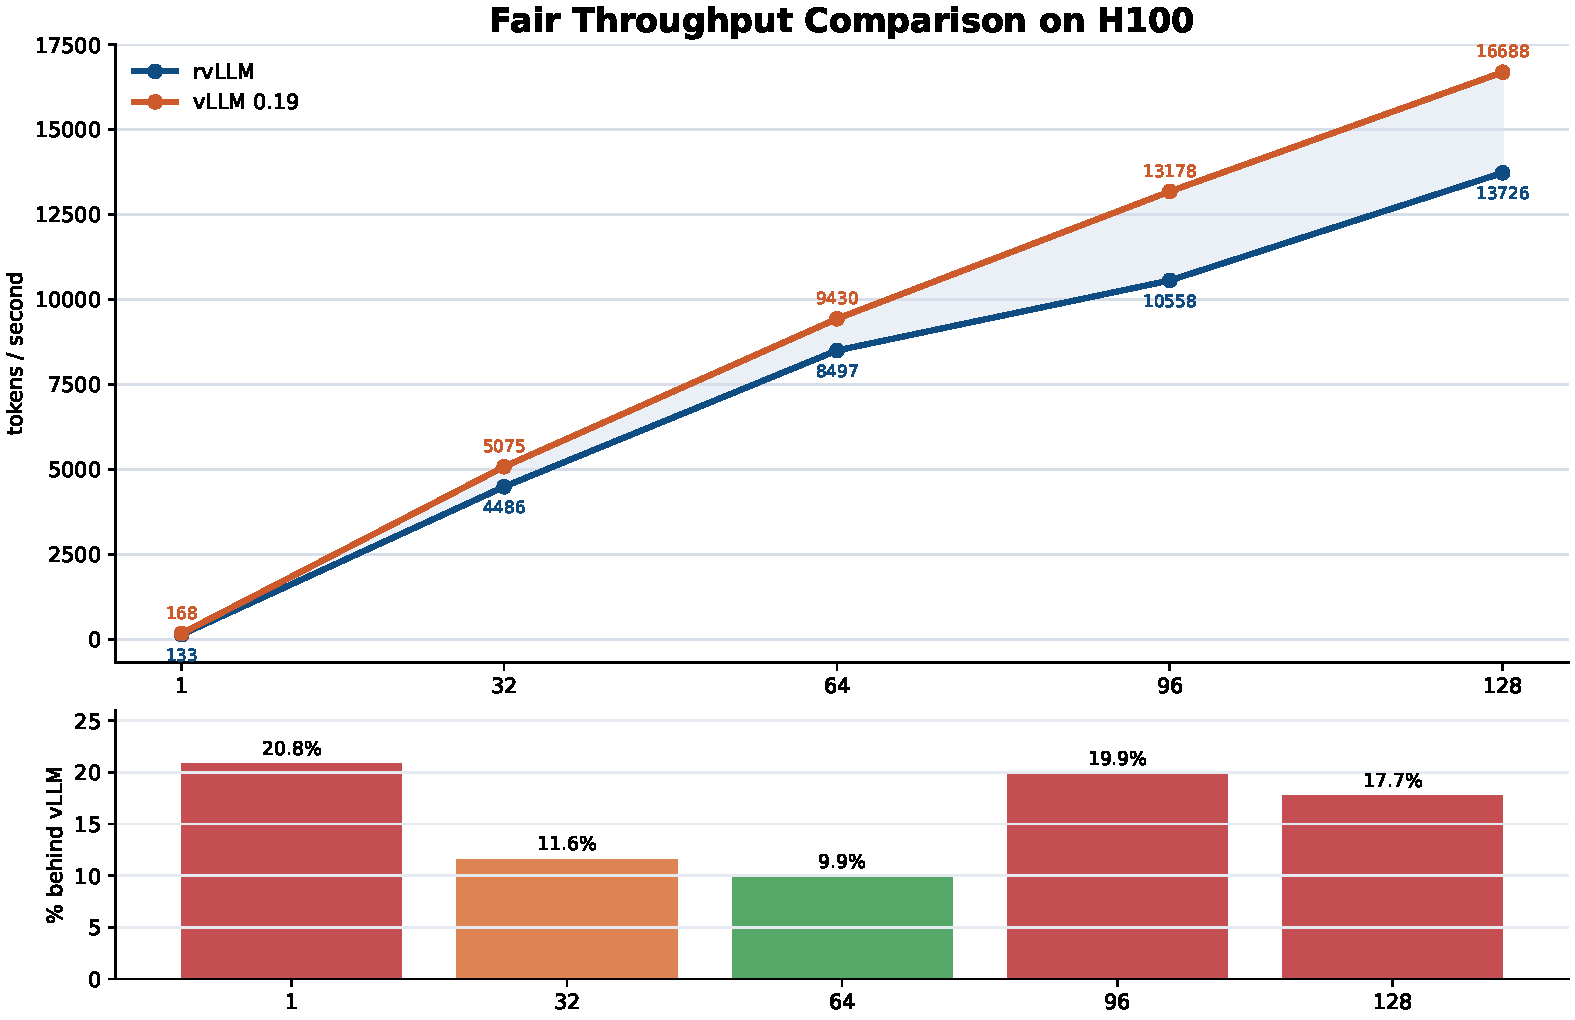
\includegraphics[width=\linewidth]{throughput_gap.pdf}
\caption{Fair throughput comparison across concurrency points, plus the relative gap to vLLM.}
\end{figure}

\section{GPU Hotspot View}

\begin{figure}[h]
\centering
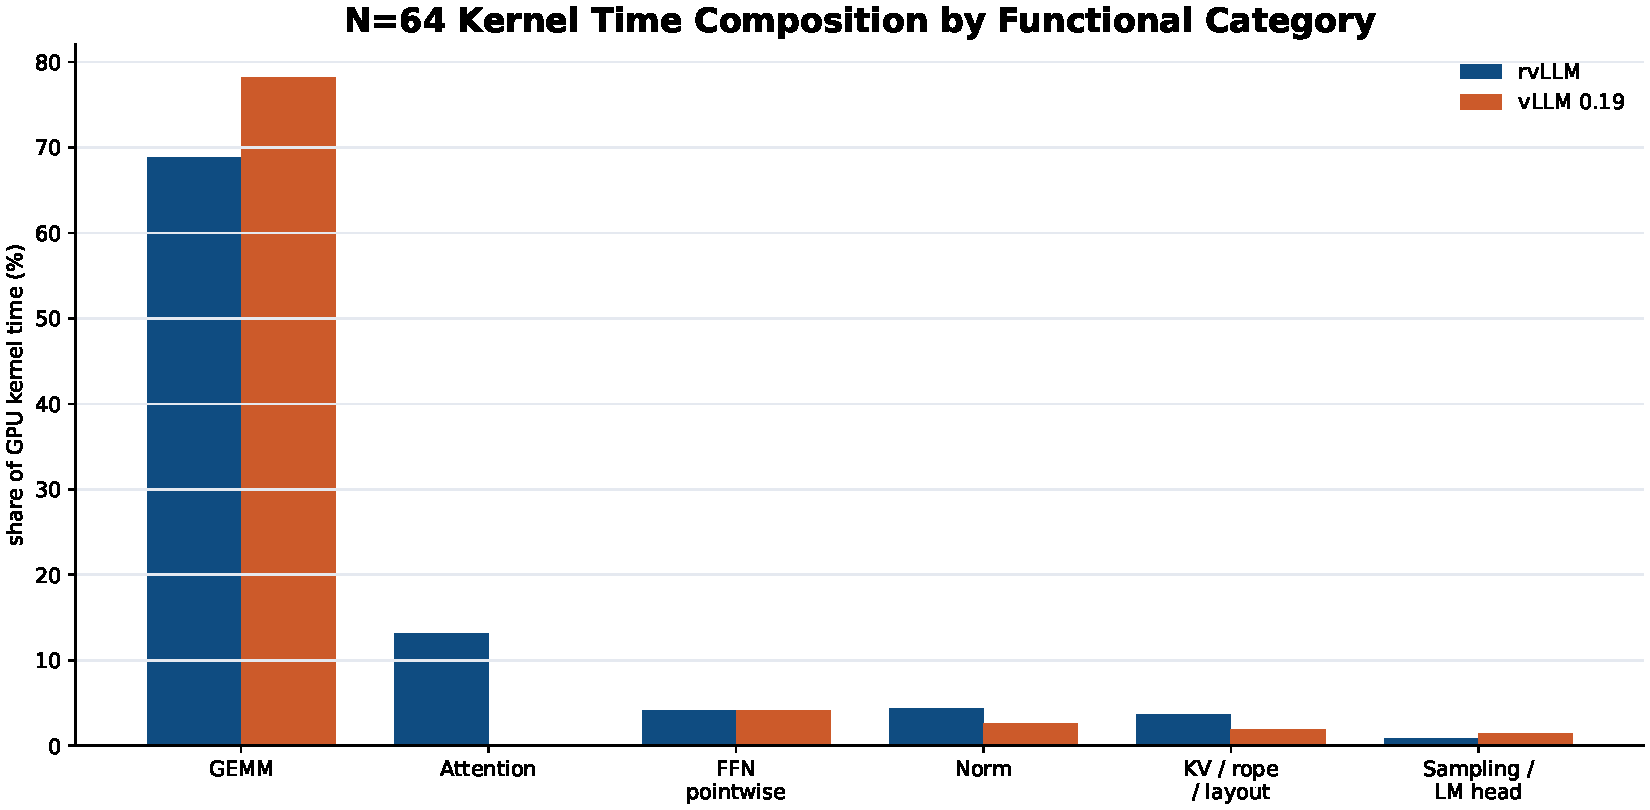
\includegraphics[width=\linewidth]{kernel_categories.pdf}
\caption{N=64 GPU kernel time grouped into comparable functional categories. vLLM spends more of its time in larger GEMM kernels and fused pointwise work. rvLLM still carries more fragmented attention, norm, and SiLU-side cost.}
\end{figure}

\reportbox{
\textbf{Read on N=64.}
rvLLM's most visible kernels are \texttt{fa3\_v3\_decode\_gqa\_kernel}, \texttt{nvjet\_hsh\_*}, \texttt{fused\_residual\_rmsnorm\_f16\_kernel}, and \texttt{silu\_mul\_interleaved\_f16\_kernel}. vLLM's profile is led by larger \texttt{nvjet\_tst\_*} GEMMs, \texttt{triton\_poi\_fused\_mul\_silu\_slice\_1}, \texttt{FlashAttnFwdSm90}, and cache update kernels. That is the core shape difference behind the remaining gap.
}

\section{Benchmark Figure}

\begin{figure}[h]
\centering
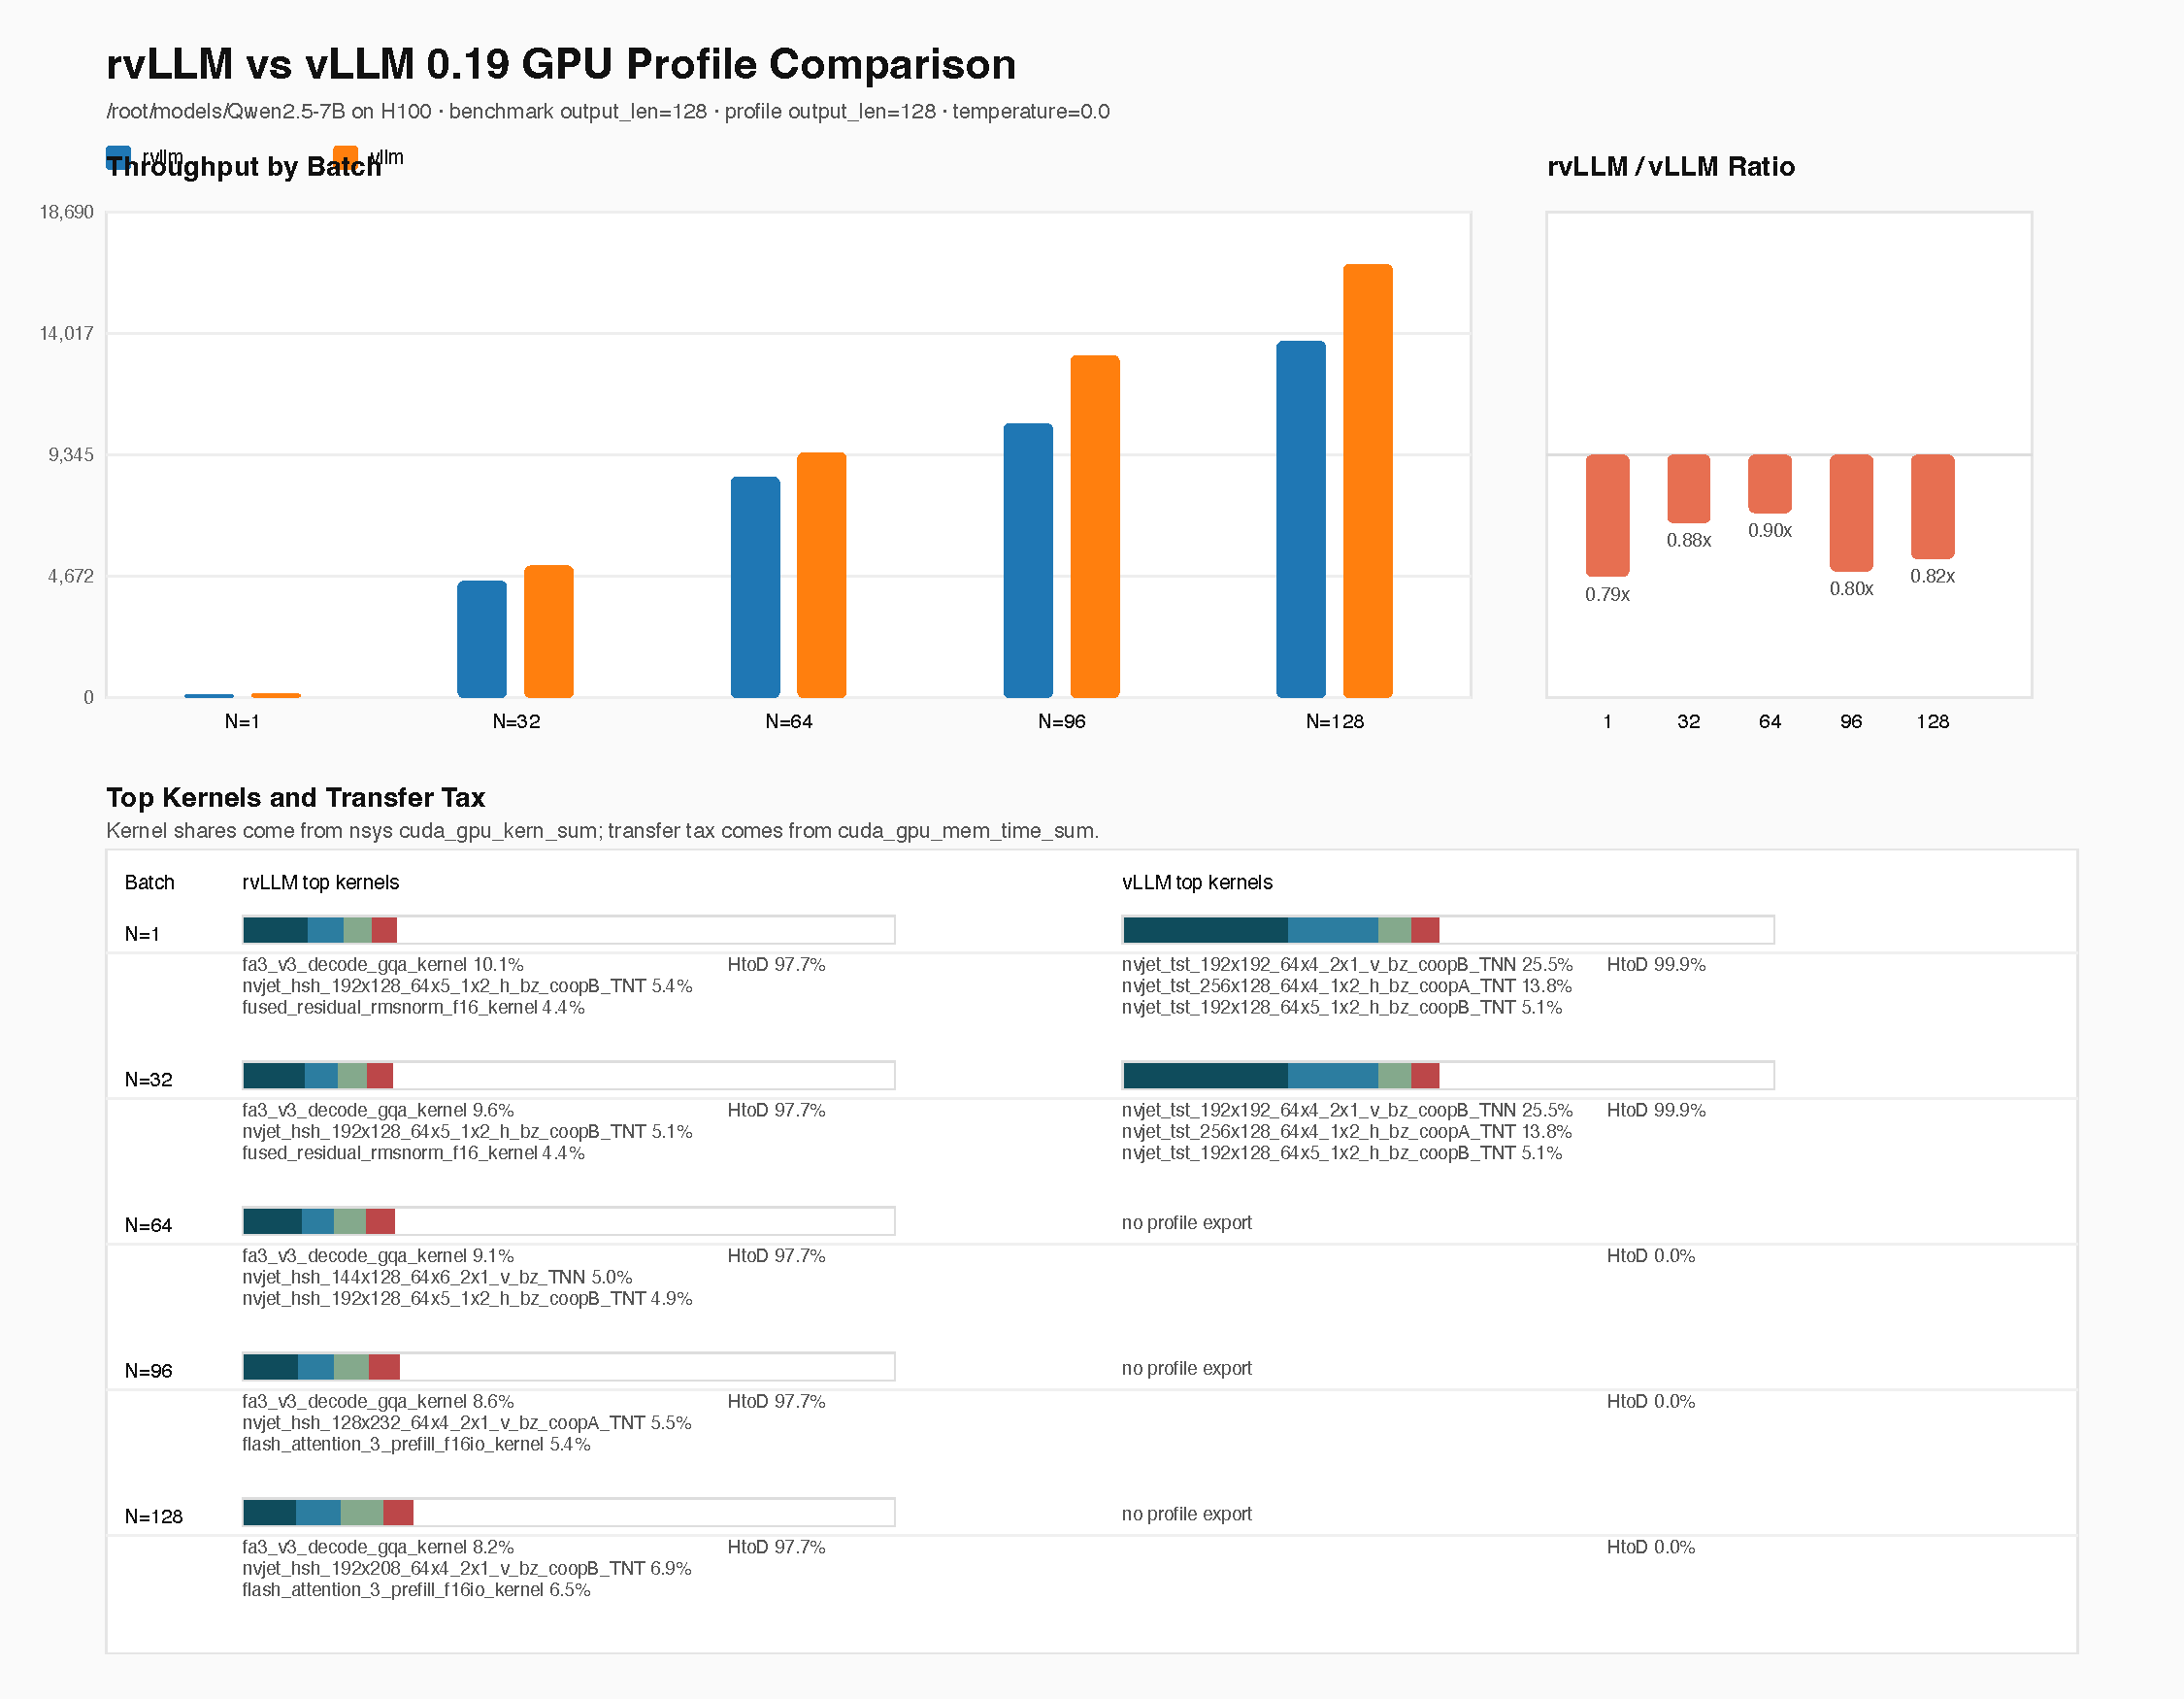
\includegraphics[width=\linewidth]{profile_compare.pdf}
\caption{Full benchmark comparison figure from the fair H100 run.}
\end{figure}

\clearpage
\section{Flamegraph}

\begin{figure}[h]
\centering
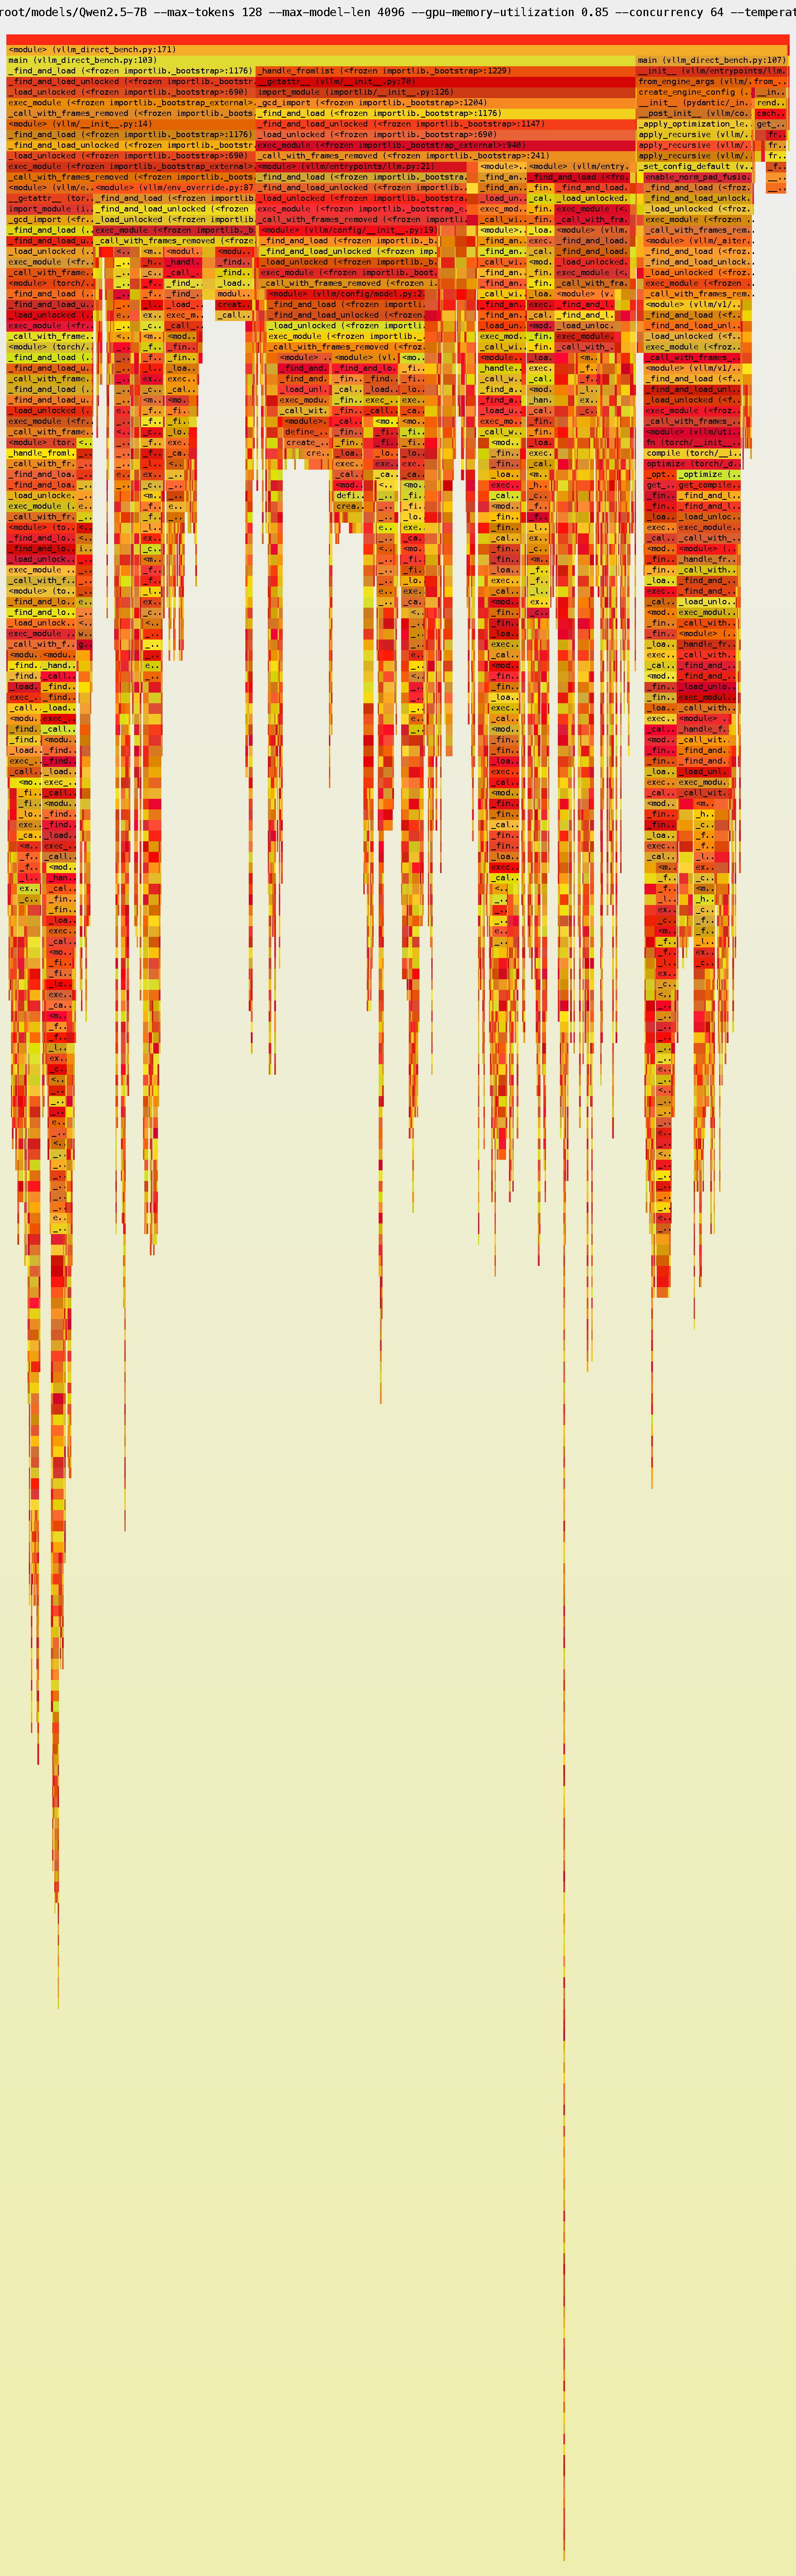
\includegraphics[width=\linewidth,height=0.86\textheight,keepaspectratio]{vllm_n64_cpu.pdf}
\caption{vLLM N=64 CPU flamegraph captured during the matched direct benchmark run.}
\end{figure}

\clearpage
\section{Notes}

\begin{itemize}
\item This report uses the fair matched benchmark run and the clean direct vLLM N=64 profile collected locally under \texttt{reports/full\_stack\_compare\_20260407}.
\item The deep rvLLM Nsight Compute pass is being collected separately because the Nsight injection path required a compatibility shim to avoid crashing on startup.
\item Once that deep pass completes, the same layout can be refreshed with Nsight Compute sections for both systems.
\end{itemize}

\end{document}
